\section{Applikationssicherheit unter iOS}
	Mobile Betriebssysteme bauen zum größten Teil auf Applikationen - weiter
	\textsl{Apps} genannt - auf, welche die produktive Nutzung eines mobilen
	Endgerätes erheblich verbessern können. Dabei ist es allerdings
	essentiell, dass diese Apps korrekt vom Betriebssystem behandelt werden, da
	andernfalls die Systemsicherheit, die Stabilität oder gar die Nutzerdaten
	gefährdet werden können. Wie bereits im Kapitel Systemsicherheit (siehe:
	\ref{sec:components-syssec}) vorgestellt, wird auch hier eine Art
	Schichtensystem angewendet, um eine Signierung und Verifikation, sowie ein
	Sandboxing der Apps sicherzustellen.
	
	\subsection{Signieren von Applikationen}
		Nach dem Start des iOS Kernels, stellt dieser sicher, welche Nutzerprozesse
		und Apps gestartet werden dürfen. Dazu werden diese auf eine Signierung durch
		ein von Apple ausgestelltes Zerifikat geprüft. Das zwingende Vorhandensein
		dieses Zertifikats stellt eine Adaption der \textsl{chain of trust} (siehe:
		\ref{sec:secure-boot-chain}) auf die Applikationsebene dar. So muss jeder
		private Entwickler als auch jedes Unternehmen seine Identität bei Apple
		verifizieren, bevor ein Entwicklerzertifikat von Apple für diese ausgestellt
		wird. Somit ist sicher gestellt, dass jede App im AppStore auf eine
		Privatperson zurückzuführen ist, was auch ein gesteigertes Vertrauen der
		Nutzer in die Qualität der Apps zur Folge hat.\\
		Allerdings muss an diesem Punkt erwähnt werden, dass Apple Ausnahmen dieser
		Verifikation in Form des \textsl{iOS Developer Enterprise
		Program}\footnote{https://developer.apple.com/programs/ios/enterprise/}
		erlaubt und so Apps auch ohne das Veröffentlichen im AppStore auf iOS Geräte
		installiert werden können. Dabei prüft Apple das anfragende Unternehmen auf
		Eignung durch deren D-U-N-S Nummer - einem Zahlensystem zur eindeutigen
		Identifizierung von Firmen. Populär wurde eine jüngste Ausnutzung dieses
		Privileges, bei welcher über eine Webseite bei Einwilligung eine App
		installiert wird, welche dann ein Abonnement verkaufen will
		\footnote{http://heise.de/-2679222}. Apple dachte diese Möglichkeit nur für
		Firmen, die ihr eigenes Mobile Device Management betreiben, an. Hier wurde
		also entweder der ausstellende Account gekapert oder diese Lizenz vom
		Eigentümer schlichtweg missbraucht.\\
		Ab iOS 8 wird es Entwicklern erlaubt in ihren Apps Frameworks zu verwenden. Um
		hier ein Laden von unsigniertem Code zu verhindern, wird beim Start einer App
		die \textsl{Team-ID} geprüft - ein 10 stelliger alphanumerischer String,
		welcher aus dem von Apple ausgestellten Entwicklerzertifikat extrahiert wird.
		Eine App darf nur Code laden, welcher entweder vom System kommt, oder die selbe
		Team-ID besitzt. Weiterhin ist es unter iOS untersagt Apps von ungeprüften
		Drittanbietern zu installieren. Dazu wird vom System zur Laufzeit die
		Signatur der App mit denen der letzten Änderung verglichen.
		
	\subsection{Schutz zur Laufzeit}
		Apple realisierte mehrere Sicherheitsmaßnahmen, um Applikationen und System zu
		schützen. In diesem Kapitel werde ich diese erläutern.
		
		\subsubsection{Sandboxing} 
			Sobald eine App erfolgreich durch einen gültigen Author verifiziert wurde,
			wird von iOS eine \textsl{Sandbox} geschaffen, was die Domäne der App
			darstellt. Alle Drittanbieter und die meisten Systemapps laufen unter dem
			Unix Benutzer \textsl{mobile}, welcher mit minimalen Rechten ausgestattet
			ist.
			\begin{figure}[h]
				\centering
				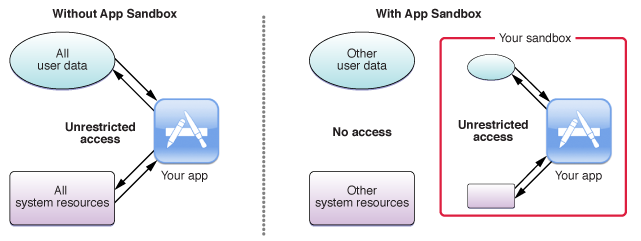
\includegraphics[width=0.9\linewidth]{ios/media/sandboxing.png}
				\caption{Sandboxing unter iOS \cite{IOSSandboxing}}
				\label{fig:sandboxing}
			\end{figure}
			Von dort ist es ihr nicht möglich Daten anderer Drittanbieter- oder
			Systemapps zu erreichen. Jede App hat ein bei der Installation zufällig
			zugewieses Home-Verzeichnis, in welchem Sie ihre Dateien hält. Wenn
			andere als die eigenen Daten benötigt werden, wird dies nur mit vom System
			vorgeschriebenen APIs ermöglicht. Zu Beginn war dies offiziell nicht
			vorgesehen und so hat sich die Entwicklergemeinde selbst einen Weg in Form von
			\textsl{URL-Schemas} gebahnt. Später kam eine weitere Möglichkeit mit dem
			Nutzen einer gemeinsamen \textsl{Key-Chain} pro AppGroup
			dazu\cite[S.83]{Banks2015}.\\%TODO: ref to AppGroups
				
		\subsubsection{Entitlements}
			Einen weiteren Schutz zur Laufzeit stellen sogenannte \textsl{Entitlements}
			dar, mit denen der Zugriff auf iCloud, Push	Notifications und
			Nutzerinformationen geregelt wird. Da diese digital signiert sind, können Sie
			nicht verändert werden. Systemapps und Hintergrundprozesse nutzen diese
			Berechtigung besonders oft, da dies verhindert, dass der relevante Prozess als
			root laufen muss. Zusätzlich verringert dies das Risiko einer ungewollten
			Rechteerweiterung durch einen manipulierten Hintergrundprozess oder einer
			Systemapp.\\
		
		\subsubsection{ASLR}
			Für zusätzlichen Laufzeitschutz wurde \textsl{Address space layout
			randomization}\cite{iOS4SecurityEvalutaion} ab iOS 4.3 eingeführt. Dies weist
			Programmen zufällige Speicheradressen zu. Somit sollen Angriffe die auf
			Speicherüberläufen basieren verhindert werden\cite[S.131]{Levin2012}. Jedoch
			wird nur der Heap und die Bibliotheken der App durch ASLR geschützt, wenn
			die App nicht mit einer Unterstützung für \textsl{Position Independent
			Executables} compiliert wurde.
			\begin{figure}[h]
				\centering
				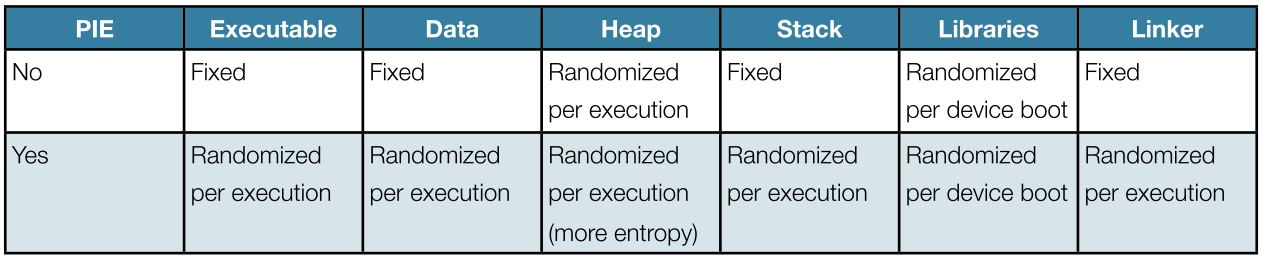
\includegraphics[width=0.9\linewidth]{ios/media/aslr-pie.jpg}
				\caption{ASLR in Abhängigkeit von PIE
				\cite{iOS4SecurityEvalutaion}}
				\label{fig:aslr}
			\end{figure}\\
		
		\subsubsection{ARM Never eXecute}
			Mit dem \textsl{NX-Bit} markiert iOS einzelne Speicherseiten entweder mit dem
			\textsl{Code-Flag} oder mit dem \textsl{Data-Flag}. Speicherseiten mit
			Data-Markierung starten einen \textsl{Page-Fault}, wenn ein Programm in
			diesem nicht ausführbaren Speicherbereich versucht eine Adresse auszuführen
			- was bedeuted, dass der Instruction Pointer versucht diesen Bereich
			aufzurufen. Dieser Seitenfehler wird von iOS registriert und damit die
			Ausführung des Programmes unterbunden\cite[S.310]{Levin2012}.
